\documentclass[tikz,border=8pt]{standalone}
\usepackage[utf8]{inputenc}
\usepackage[T1]{fontenc}
\usepackage{amsmath,amssymb}
\usetikzlibrary{arrows.meta,positioning,calc,shapes.geometric}

\definecolor{bgdark}{HTML}{0F172A}
\definecolor{paneldark}{HTML}{1E293B}
\definecolor{gridline}{HTML}{334155}
\definecolor{cellbg}{HTML}{0B1120}
\definecolor{agentblue}{HTML}{38BDF8}
\definecolor{obsred}{HTML}{EF4444}
\definecolor{goalgreen}{HTML}{22C55E}
\definecolor{threatamber}{HTML}{F59E0B}
\definecolor{mirrorpurple}{HTML}{A855F7}
\definecolor{textlight}{HTML}{F8FAFC}
\definecolor{textmuted}{HTML}{94A3B8}

% Helper macro for an 8x8 panel
\newcommand{\drawpanelgrid}[2]{
    \fill[paneldark, rounded corners=6pt] (-0.70, -2.75) rectangle (8.70, 9.15);
    \draw[gridline, line width=0.8pt, rounded corners=6pt] (-0.70, -2.75) rectangle (8.70, 9.15);
    \node[anchor=west, text=textlight, font=\sffamily\bfseries\scriptsize] at (-0.48, 8.78) {#1};
    \node[anchor=west, text=textmuted, font=\sffamily\tiny] at (-0.48, 8.40) {#2};

    \fill[cellbg] (0, 0) rectangle (8, 8);
    \draw[gridline, line width=0.45pt] (0, 0) grid (8, 8);
    \draw[gridline, line width=0.9pt] (0, 0) rectangle (8, 8);

    \foreach \i in {0,...,7} {
        \node[text=textmuted, font=\sffamily\tiny] at (\i+0.5, 8.15) {\i};
        \node[text=textmuted, font=\sffamily\tiny] at (-0.22, 7.5-\i) {\i};
    }
}

% Draw obstacle at (#1=row, #2=col)
\newcommand{\drawobs}[2]{
    \pgfmathsetmacro{\ox}{#2}
    \pgfmathsetmacro{\oy}{7-#1}
    \fill[obsred, rounded corners=2.0pt] (\ox+0.20, \oy+0.20) rectangle (\ox+0.80, \oy+0.80);
}

% Draw agent at (#1=row, #2=col, #3=theta: 0=N, 1=E, 2=S, 3=W, #4=color)
\newcommand{\drawagentcol}[4]{
    \pgfmathsetmacro{\ax}{#2+0.5}
    \pgfmathsetmacro{\ay}{7-#1+0.5}
    \pgfmathsetmacro{\rotangle}{-#3*90}
    \begin{scope}[shift={(\ax,\ay)}, rotate=\rotangle]
        \fill[#4] (0, 0.32) -- (0.26, -0.26) -- (0, -0.12) -- (-0.26, -0.26) -- cycle;
        \draw[white, line width=0.35pt] (0, 0.32) -- (0.26, -0.26) -- (0, -0.12) -- (-0.26, -0.26) -- cycle;
    \end{scope}
}

\begin{document}
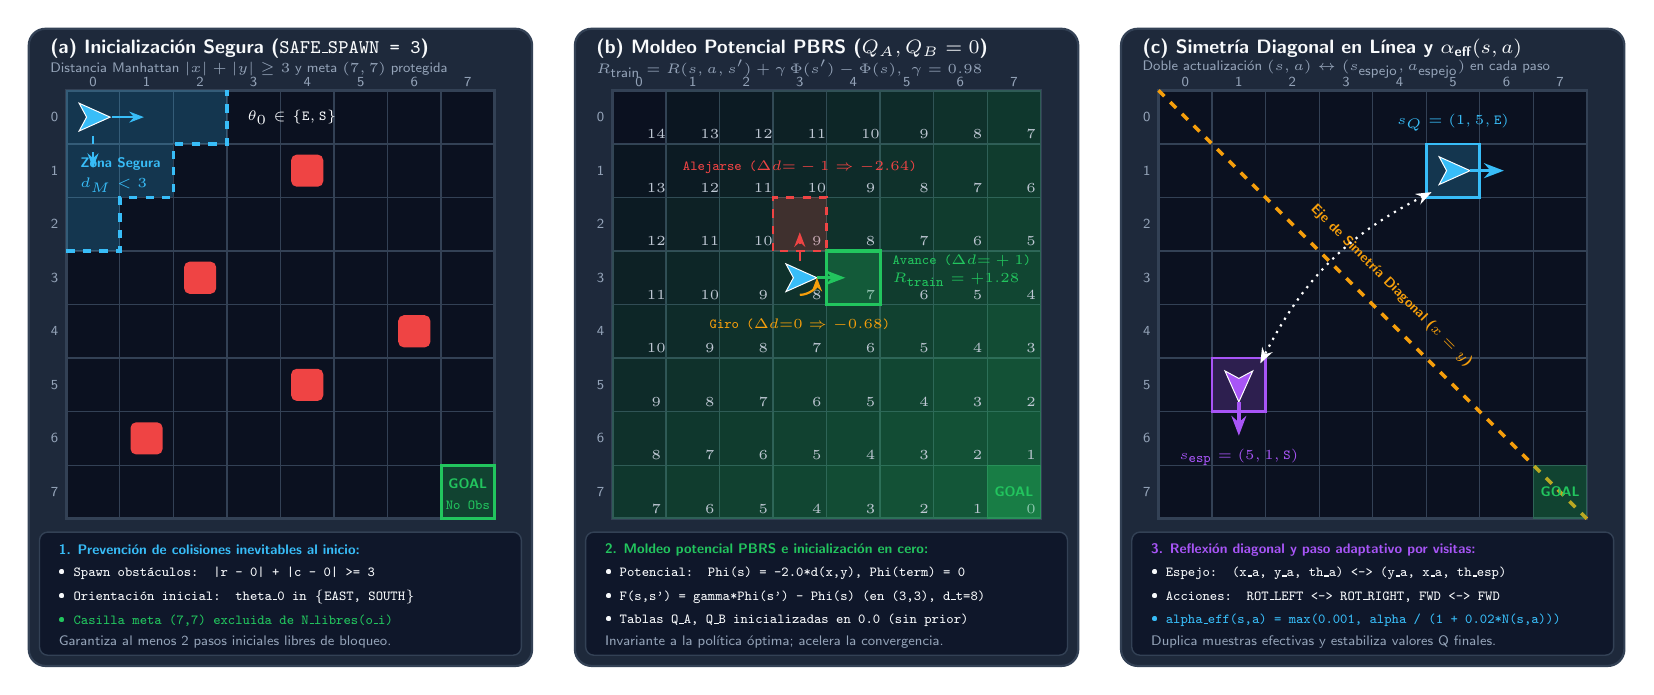
\begin{tikzpicture}[scale=0.68]

% =========================================================================
% PANEL (a): SAFE_SPAWN_DISTANCE = 3 & Goal Protection
% =========================================================================
\begin{scope}[shift={(0, 0)}]
    \drawpanelgrid{(a) Inicializaci\'on Segura (\texttt{SAFE\_SPAWN = 3})}{Distancia Manhattan $|x|+|y| \ge 3$ y meta $(7,7)$ protegida}

    % Safe zone around (0,0): cells with r + c < 3 -> (0,0), (0,1), (0,2), (1,0), (1,1), (2,0)
    \foreach \r/\c in {0/0, 0/1, 0/2, 1/0, 1/1, 2/0} {
        \pgfmathsetmacro{\sx}{\c}
        \pgfmathsetmacro{\sy}{7-\r}
        \fill[agentblue, fill opacity=0.22] (\sx, \sy) rectangle (\sx+1, \sy+1);
    }
    % Boundary line of Manhattan distance >= 3
    \draw[agentblue, dashed, line width=1.3pt] (0, 5) -- (1, 5) -- (1, 6) -- (2, 6) -- (2, 7) -- (3, 7) -- (3, 8);
    \node[anchor=north west, text=agentblue, font=\sffamily\bfseries\tiny] at (0.08, 6.92) {Zona Segura};
    \node[anchor=north west, text=agentblue, font=\ttfamily\tiny] at (0.08, 6.55) {$d_M < 3$};

    % Goal cell (7,7) protected
    \fill[goalgreen, fill opacity=0.28] (7, 0) rectangle (8, 1);
    \draw[goalgreen, line width=1.1pt] (7, 0) rectangle (8, 1);
    \node[text=goalgreen, font=\sffamily\bfseries\tiny] at (7.5, 0.65) {GOAL};
    \node[text=goalgreen, font=\ttfamily\tiny] at (7.5, 0.25) {No Obs};

    % Valid obstacle spawn zone example
    \drawobs{1}{4}
    \drawobs{3}{2}
    \drawobs{4}{6}
    \drawobs{6}{1}
    \drawobs{5}{4}

    % Agent at (0,0) with initial theta in {EAST, SOUTH}
    \drawagentcol{0}{0}{1}{agentblue}
    \draw[-{Stealth[scale=0.8]}, agentblue, thick] (0.85, 7.5) -- (1.45, 7.5);
    \draw[-{Stealth[scale=0.8]}, agentblue, thick, dashed] (0.5, 7.15) -- (0.5, 6.55);
    \node[anchor=west, text=textlight, font=\ttfamily\tiny] at (3.2, 7.5) {$\theta_0 \in \{\text{E}, \text{S}\}$};

    % Bottom explanation box
    \fill[bgdark, rounded corners=3pt] (-0.50, -2.55) rectangle (8.50, -0.25);
    \draw[gridline, line width=0.5pt, rounded corners=3pt] (-0.50, -2.55) rectangle (8.50, -0.25);
    \node[anchor=west, text=agentblue, font=\sffamily\bfseries\tiny] at (-0.32, -0.58) {1. Prevenci\'on de colisiones inevitables al inicio:};
    \node[anchor=west, text=textlight, font=\ttfamily\tiny] at (-0.32, -1.02) {• Spawn obst\'aculos: |r - 0| + |c - 0| >= 3};
    \node[anchor=west, text=textlight, font=\ttfamily\tiny] at (-0.32, -1.46) {• Orientaci\'on inicial: theta\_0 in \{EAST, SOUTH\}};
    \node[anchor=west, text=goalgreen, font=\ttfamily\tiny] at (-0.32, -1.90) {• Casilla meta (7,7) excluida de N\_libres(o\_i)};
    \node[anchor=west, text=textmuted, font=\sffamily\tiny] at (-0.32, -2.30) {Garantiza al menos 2 pasos iniciales libres de bloqueo.};
\end{scope}

% =========================================================================
% PANEL (b): Discounted Potential-Based Reward Shaping (PBRS) & Zero Init
% =========================================================================
\begin{scope}[shift={(10.2, 0)}]
    \drawpanelgrid{(b) Moldeo Potencial PBRS ($Q_A, Q_B = 0$)}{$R_{\text{train}} = R(s,a,s') + \gamma\,\Phi(s') - \Phi(s),\ \gamma=0.98$}

    % Heatmap shading of Manhattan distance d = (7-r) + (7-c)
    \foreach \r in {0,...,7} {
        \foreach \c in {0,...,7} {
            \pgfmathsetmacro{\dist}{(7-\r)+(7-\c)}
            \pgfmathsetmacro{\op}{0.03*(14-\dist)}
            \pgfmathsetmacro{\cx}{\c}
            \pgfmathsetmacro{\cy}{7-\r}
            \fill[goalgreen, fill opacity=\op] (\cx, \cy) rectangle (\cx+1, \cy+1);
            \node[text=textmuted!60, font=\ttfamily\tiny] at (\cx+0.82, \cy+0.18) {\pgfmathprintnumber[int trunc]{\dist}};
        }
    }
    \fill[goalgreen, fill opacity=0.32] (7, 0) rectangle (8, 1);
    \node[text=goalgreen, font=\sffamily\bfseries\tiny] at (7.5, 0.5) {GOAL};

    % Agent at (3,3) facing EAST (theta=1), d_t=8, Phi(s)=-16.0
    \drawagentcol{3}{3}{1}{agentblue}

    % Case 1: Advance toward goal (3,3)->(3,4), d_{t+1}=7 -> R_train = -1 + 0.98(-14) - (-16) = +1.28
    \fill[goalgreen, fill opacity=0.25] (4, 4) rectangle (5, 5);
    \draw[goalgreen, line width=1.1pt] (4, 4) rectangle (5, 5);
    \draw[-{Stealth[scale=0.85]}, goalgreen, very thick] (3.82, 4.5) -- (4.35, 4.5);
    \node[anchor=west, text=goalgreen, font=\ttfamily\bfseries\tiny] at (5.05, 4.82) {Avance ($\Delta d{=}+1$)};
    \node[anchor=west, text=goalgreen, font=\ttfamily\tiny] at (5.05, 4.46) {$R_{\text{train}} = +1.28$};

    % Case 2: Rotate in place at (3,3), d_{t+1}=8 -> R_train = -1 + 0.98(-16) - (-16) = -0.68
    \draw[-{Stealth[scale=0.75]}, threatamber, thick] (3.5, 4.18) arc (-90:0:0.32);
    \node[anchor=north, text=threatamber, font=\ttfamily\bfseries\tiny] at (3.5, 3.92) {Giro ($\Delta d{=}0 \Rightarrow -0.68$)};

    % Case 3: Move away from goal (3,3)->(2,3), d_{t+1}=9 -> R_train = -1 + 0.98(-18) - (-16) = -2.64
    \fill[obsred, fill opacity=0.22] (3, 5) rectangle (4, 6);
    \draw[obsred, dashed, line width=0.9pt] (3, 5) rectangle (4, 6);
    \draw[-{Stealth[scale=0.8]}, obsred, thick, dashed] (3.5, 4.82) -- (3.5, 5.35);
    \node[anchor=south, text=obsred, font=\ttfamily\bfseries\tiny] at (3.5, 6.26) {Alejarse ($\Delta d{=}-1 \Rightarrow -2.64$)};

    % Bottom explanation box
    \fill[bgdark, rounded corners=3pt] (-0.50, -2.55) rectangle (8.50, -0.25);
    \draw[gridline, line width=0.5pt, rounded corners=3pt] (-0.50, -2.55) rectangle (8.50, -0.25);
    \node[anchor=west, text=goalgreen, font=\sffamily\bfseries\tiny] at (-0.32, -0.58) {2. Moldeo potencial PBRS e inicializaci\'on en cero:};
    \node[anchor=west, text=textlight, font=\ttfamily\tiny] at (-0.32, -1.02) {• Potencial: Phi(s) = -2.0*d(x,y), Phi(term) = 0};
    \node[anchor=west, text=textlight, font=\ttfamily\tiny] at (-0.32, -1.46) {• F(s,s') = gamma*Phi(s') - Phi(s) (en (3,3), d\_t=8)};
    \node[anchor=west, text=textlight, font=\ttfamily\tiny] at (-0.32, -1.90) {• Tablas Q\_A, Q\_B inicializadas en 0.0 (sin prior)};
    \node[anchor=west, text=textmuted, font=\sffamily\tiny] at (-0.32, -2.30) {Invariante a la pol\'itica \'optima; acelera la convergencia.};
\end{scope}

% =========================================================================
% PANEL (c): Online Diagonal Symmetry & Adaptive Alpha
% =========================================================================
\begin{scope}[shift={(20.4, 0)}]
    \drawpanelgrid{(c) Simetr\'ia Diagonal en L\'inea y $\alpha_{\text{eff}}(s,a)$}{Doble actualizaci\'on $(s,a) \leftrightarrow (s_{\text{espejo}}, a_{\text{espejo}})$ en cada paso}

    % Main diagonal line from (0,0) [top-left=(0,8)] to (7,7) [bottom-right=(8,0)]
    \draw[threatamber, dashed, line width=1.3pt] (0, 8) -- (8, 0);
    \node[text=threatamber, font=\sffamily\bfseries\tiny, rotate=-45] at (4.35, 4.35) {Eje de Simetr\'ia Diagonal ($x = y$)};

    % Original state s_Q at (x_a=1, y_a=5, theta_a=E)
    \fill[agentblue, fill opacity=0.22] (5, 6) rectangle (6, 7);
    \draw[agentblue, line width=1.0pt] (5, 6) rectangle (6, 7);
    \drawagentcol{1}{5}{1}{agentblue}
    \draw[-{Stealth[scale=0.85]}, agentblue, very thick] (5.82, 6.5) -- (6.45, 6.5);
    \node[anchor=south, text=agentblue, font=\ttfamily\bfseries\tiny] at (5.5, 7.05) {$s_Q=(1,5,\text{E})$};

    % Mirror state s_esp at (x_a=5, y_a=1, theta_a=S)
    \fill[mirrorpurple, fill opacity=0.22] (1, 2) rectangle (2, 3);
    \draw[mirrorpurple, line width=1.0pt] (1, 2) rectangle (2, 3);
    \drawagentcol{5}{1}{2}{mirrorpurple}
    \draw[-{Stealth[scale=0.85]}, mirrorpurple, very thick] (1.5, 2.18) -- (1.5, 1.55);
    \node[anchor=north, text=mirrorpurple, font=\ttfamily\bfseries\tiny] at (1.5, 1.48) {$s_{\text{esp}}=(5,1,\text{S})$};

    % Bidirectional reflection arrow across the diagonal
    \draw[{Stealth[scale=0.85]}-{Stealth[scale=0.85]}, white!85, thick, dotted] (5.1, 6.1) to[bend right=18] (1.9, 2.9);

    % Goal cell (7,7)
    \fill[goalgreen, fill opacity=0.28] (7, 0) rectangle (8, 1);
    \node[text=goalgreen, font=\sffamily\bfseries\tiny] at (7.5, 0.5) {GOAL};

    % Bottom explanation box
    \fill[bgdark, rounded corners=3pt] (-0.50, -2.55) rectangle (8.50, -0.25);
    \draw[gridline, line width=0.5pt, rounded corners=3pt] (-0.50, -2.55) rectangle (8.50, -0.25);
    \node[anchor=west, text=mirrorpurple, font=\sffamily\bfseries\tiny] at (-0.32, -0.58) {3. Reflexi\'on diagonal y paso adaptativo por visitas:};
    \node[anchor=west, text=textlight, font=\ttfamily\tiny] at (-0.32, -1.02) {• Espejo: (x\_a, y\_a, th\_a) <-> (y\_a, x\_a, th\_esp)};
    \node[anchor=west, text=textlight, font=\ttfamily\tiny] at (-0.32, -1.46) {• Acciones: ROT\_LEFT <-> ROT\_RIGHT, FWD <-> FWD};
    \node[anchor=west, text=agentblue, font=\ttfamily\tiny] at (-0.32, -1.90) {• alpha\_eff(s,a) = max(0.001, alpha / (1 + 0.02*N(s,a)))};
    \node[anchor=west, text=textmuted, font=\sffamily\tiny] at (-0.32, -2.30) {Duplica muestras efectivas y estabiliza valores Q finales.};
\end{scope}

\end{tikzpicture}
\end{document}
